% This file was created (at least in part) by the script ParseMdtoLatex by Louis du Plessis
% (Available from https://github.com/taming-the-beast)

\documentclass[11pt]{article}
\input{preamble}

% Add your bibtex library here
\addbibresource{master-refs}


%%%%%%%%%%%%%%%%%%%%
% Do NOT edit this %
%%%%%%%%%%%%%%%%%%%%
\begin{document}
\renewcommand{\headrulewidth}{0.5pt}
\headsep = 20pt
\lhead{ }
\rhead{\textsc {BEAST v2 Tutorial}}
\thispagestyle{plain}


%%%%%%%%%%%%%%%%%%
% Tutorial title %
%%%%%%%%%%%%%%%%%%
\begin{center}

	% Enter the name of your tutorial here
	\textbf{\LARGE Tutorial using BEAST v2.4.2}\\\vspace{2mm}

	% Enter a short description of your tutorial here
	\textbf{\textcolor{mycol}{\Large Skyline plots}}\\

	\vspace{4mm}

	% Enter the names of all the authors here
	{\Large {\em Nicola F. Müller and Louis du Plessis}}
\end{center}

Inference of past population dynamics using Bayesian Coalescent Skyline
and Birth-Death Skyline plots.

%%%%%%%%%%%%%%%%%
% Tutorial body %
%%%%%%%%%%%%%%%%%

\section{Background}\label{background}

Population dynamics influence the shape of the tree and consequently,
the shape of the tree contains some information about past population
dynamics. The so-called Skyline methods allow to extract this
information from phylogenetic trees in a non-parametric manner. It is
non-parametric since there is no underlying system of differential
equations governing the inference of these dynamics. In this tutorial we
will look at two different methods to infer these dynamics from sequence
data. The first one is the Bayesian Coalescent Skyline plot
\citep{Drummond2005}, which is based on the coalescent model, and the
second one is the Birth-Death skyline \citep{Stadler2013} plot based on
the birth-death model. The conceptual difference between coalescent and
birth-death approaches lies in the direction of the flow of time. In the
coalescent, the time is modeled to go backwards, from present to past,
while in the birth-death approach it is modeled to go forwards. Two
other fundamental differences are the parameters that are inferred and
the way sampling is treated. \clearpage

\section{Programs used in this
Exercise}\label{programs-used-in-this-exercise}

\subsubsection{BEAST2 - Bayesian Evolutionary Analysis Sampling Trees
2}\label{beast2---bayesian-evolutionary-analysis-sampling-trees-2}

BEAST2 is a free software package for Bayesian evolutionary analysis of
molecular sequences using MCMC and strictly oriented toward inference
using rooted, time-measured phylogenetic trees \citep{Bouckaert2014}.
This tutorial uses the BEAST2 version 2.4.2.

\subsubsection{BEAUti - Bayesian Evolutionary Analysis
Utility}\label{beauti---bayesian-evolutionary-analysis-utility}

BEAUti is a graphical user interface tool for generating BEAST2 XML
configuration files.

\subsubsection{Tracer}\label{tracer}

\href{http://tree.bio.ed.ac.uk/software/tracer}{Tracer} is used to
summarise the posterior estimates of the various parameters sampled by
the Markov chain. This program can be used for visual inspection and
assessment of convergence. It helps to quickly view median estimates
95\% highest posterior density intervals of the parameters, and
calculates the effective sample sizes (ESS) of parameters. It also helps
to visualise potential parameter correlations.

\subsubsection{R}\label{r}

We will be using \href{/href\%7Bhttps://www.r-project.org}{R} to analyze
the output of the birth-death skyline plot. We will start the provided R
script from the terminal, hence there is no need for applications like
RStudio, which provides a graphical user interface for R. If you prefer
using RStudio feel free to do so. \clearpage

\section{Practical: Bayesian and birth-death skyline
plot}\label{practical-bayesian-and-birth-death-skyline-plot}

In this tutorial we will estimate the dynamics of the Egyptian Hepatitis
C epidemic from genetic sequence data collected in 1993.

The aim of this tutorial is to:

\begin{itemize}

\item
  Learn how to infer population dynamics;
\item
  Get to know how to choose the set-up of a skyline analysis;
\item
  Get to know the advantages and disadvantages of the Bayesian
  Coalescent Skyline and the Birth-Death Skyline.
\end{itemize}

\subsection{The Data}\label{the-data}

The dataset consists of an alignment of 63 Hepatitis C sequences sampled
in 1993 in Egypt \citep{Ray2000}. This dataset has been used previously
to test the performance of skyline methods
\citep{Pybus2003, Drummond2005, Stadler2013}.

With an estimated 15-25\%, Egypt has the highest Hepatits C prevalence
in the world. In the mid 20$^{th}$ century, the prevalence of Hepatitis
C increased drastically (see Figure \ref{fig:prevalence} for estimates).
We will try to infer this increase from sequence data.

\begin{figure}
    \centering
    \includegraphics[width=0.500000\textwidth]{figures/Estimated_number_hcv.png}
    \caption{The estimated number of Hepatitis C cases in Egypt \citep{Pybus2003}.}
    \label{fig:prevalence}
\end{figure}

\subsection{Creating the Analysis File with
BEAUti}\label{creating-the-analysis-file-with-beauti}

We will use BEAUti to generate the configuration file for BEAST2 from
the sequence alignment.

\subsubsection{Install BEAST 2 Plug-Ins}\label{install-beast-2-plug-ins}

While the Bayesian Coalescent Skyline plot is integrated in the core of
BEAST2, we need to install the BDSKY package, which contains the
birth-death skyline plot functionality. Installation of packages is done
using the package manager, which is integrated into BEAUti. Open the
package manager with \lstinline!File > Manage Packages! in BEAUti.
Select the BDSKY package and install it using the
\lstinline!Install/Upgrade! button (Figure \ref{fig:install}).

\begin{figure}
    \centering
    \includegraphics[width=0.500000\textwidth]{figures/install_bdsky.png}
    \caption{Install the package BDSKY which contains the birth-death skyline functionality.}
    \label{fig:install}
\end{figure}

 \clearpage

\subsubsection{Setting up the analysis with Bayesian Coalescent
Skyline}\label{setting-up-the-analysis-with-bayesian-coalescent-skyline}

To import the aligned sequences into BEAUti, use
\lstinline!File > Import Alignment! to select the \lstinline!*.nexus!
file.

BEAUti will recognize the sequences from the \lstinline!*.nexus! file as
nucleotide data. It will do so for sequence files with the character set
of \textbf{A \textbar{} C \textbar{} G \textbar{} T \textbar{} N}, where
\textbf{N} indicates an unknown nucleotide. As soon as other non-gap
characters are included (e.g.~using \textbf{R} or \textbf{Y} to indicate
purines and pyramidines) BEAUti will not recognize the data as
nucleotides anymore, unless the type of data is specified in the
\lstinline!*.nexus! file.

After we have loaded the sequences into BEAUti, we have to specify the
evolutionary model. We will be using the very general GTR model (Figure
\ref{fig:model}), which estimates transition probabilities between
individual nucleotides separately, meaning that transition probabilities
between e.g. \textbf{A} and \textbf{T} will be inferred separately to
the ones between \textbf{A} and \textbf{C}. Additionally, we should
allow for rate heterogeneity among sites. We can do this by changing the
Gamma Category Count to 4 (normally between 4 and 6).

\begin{figure}
    \centering
    \includegraphics[max width=\textwidth, max height=0.9\textheight]{figures/choose_gtr.png}
    \caption{Set GTR as a site model. Also use a Gamma Category Count of 4.}
    \label{fig:model}
\end{figure}

As we use sequences that were sampled at the same point in time, we need
to fix the clock rate (for more information on this please refer to the
tutorial on molecular clocks). We will use an estimate inferred in
\citep{Pybus2001} to fix the clock rate. In this case all the samples
were contemporaneous (at the same time) and the clock rate works as a
mapping of the estimated tree branch lengths into calendar time.

We will keep the strict clock model and will set \lstinline!Clock.rate!
to 0.00079.

Next, we need to go the the \lstinline!Priors! tab and set the Bayesian
Coalescent Skyline as a tree prior (Figure \ref{fig:coalescent}).

\begin{figure}
    \centering
    \includegraphics[max width=\textwidth, max height=0.9\textheight]{figures/choose_coalescentSkyline.png}
    \caption{Choose the Coalescent Bayesian Skyline as a population prior.}
    \label{fig:coalescent}
\end{figure}

The Bayesian Coalescent Skyline works by dividing the time between the
present and the root of the tree into intervals, thus the number of
these intervals has to be defined. Each interval will have a different
effective population size. The Bayesian Coalescent Skyline will estimate
the number of coalescent events within each interval (which is captured
in the Group Size parameter) as well as the effective population size
for that interval. The number of intervals is equal to the dimension
specified. If we have $ d $ intervals, the effective
population size is allowed to change $ d-1 $ times. To
specify the number of dimensions, we need to first go to the
initialization panel. This is by default not visible
\lstinline!View > Show Initialization Panel!.

For this analysis we will set the number of dimensions to 4 (the default
value is 5). Keep in mind that one has to change the dimension of
\lstinline!bPopSizes! as well as \lstinline!bGroupSizes!. The dimension
of both parameters has to be the same (Figure \ref{fig:dimensions}).

\begin{figure}
    \centering
    \includegraphics[max width=\textwidth, max height=0.9\textheight]{figures/set_dimension.png}
    \caption{Set the dimension of the two parameters, bPopSizes and bGroupSizes, to 4.}
    \label{fig:dimensions}
\end{figure}

Choosing the dimension for the Bayesian Coalescent Skyline can be rather
arbitrary. If the dimension is chosen too low, not all population
changes are captured, if it is chosen too large, there might be too
little information in an interval to support an estimate of a population
size. There are implementations in BEAST of the coalescent skyline that
either sample dimensions (Extended Bayesian Skyline \citep{Heled2008})
or do not require dimensions to be specified (Skyride
\citep{Minin2008}).

We can leave the priors as they are and save the settings to
\lstinline!*.xml!.

\subsubsection{Effective Population
Size}\label{effective-population-size}

The effective population size is the inverse of the rate of coalescence
$ \lambda $. The larger the effective population size
$ N_{\mathrm{eff}} $ the less likely lineages are to
coalesce.

\begin{equation}
    \lambda = \frac{1}{N_{\mathrm{eff}}}
\end{equation}

For an SIR model (\textbf{S}usceptible, \textbf{I}nfected and
\textbf{R}ecovered), it is proportional to the overall population size
$ N $ and the number of infected $ I $ and
inversely proportional to the transmission rate $ \theta $.

\begin{equation}
    N_{\mathrm{eff}} = \frac{I}{\theta} \frac{N}{S}
\end{equation}

Estimates of the effective population size
$ N_{\mathrm{eff}} $ therefore do not directly tell us
something about the number of infected, nor the transmission rate.
Changes of e.g.~the transmission rate or the number of infected can show
in the effective population size (if they do not cancel out).

\begin{figure}
    \centering
    \includegraphics[width=0.500000\textwidth]{figures/coalescent_intervals.png}
    \caption{Example tree where the red dotted lines show the time-points of coalescent events.}
    \label{fig:coal_principle}
\end{figure}

What the Bayesian Coalescent Skyline is doing is dividing the full tree
into dimension $ d $ intervals between coalescent events. It
then estimates based on what happens in those intervals, what the
effective population size is (the actual estimation additionally
involves smoothing priors which restrict the difference in effective
population sizes between two intervals). The length of an interval is
therefore not a fixed value but dependent on where the coalescent events
are (Figure \ref{fig:coal_principle}, compare later to Figure
\ref{fig:bdsky_principle} for the birth-death skyline), as well as the
number of events contained within an interval (the \lstinline!GroupSize!
parameter). Intervals are grouped together, because as Figure
\ref{fig:coal_principle} shows, some of the intervals can be very small,
which may lead to erratic estimates. Grouping intervals together leads
to smoother estimates.

\subsubsection{Exploring the results of Bayesian Coalescent Skyline
analysis}\label{exploring-the-results-of-bayesian-coalescent-skyline-analysis}

For the reconstruction of the population dynamics, we need two files:
the \lstinline!*.log! file and the \lstinline!*.trees! file. The log
files contain the information about the group size and the population
size. The group size specifies how many intervals are combined to have
the same effective population size.

After the runs have finished, load the finished \lstinline!*.log! file
into Tracer. Alternatively you can use the \lstinline!*.log! files and
the \lstinline!*.trees! files you downloaded with the data. To run the
analysis, open the finished \lstinline!*.log! file into Tracer, then go
to \lstinline!Analysis > Bayesian Skyline Reconstruction!. From there
open the finished \lstinline!*.trees! file. To get the correct years in
the analysis we should specify the \lstinline!Age of the youngest tip!.
In our case it is 1993, the year where all the samples were taken. If
the samples were taken through time, the age of the youngest tip is the
time when the most recent sample was taken. If you now press the
\lstinline!Ok! button, the reconstruction of the past population
dynamics will be performed (Figure \ref{fig:trees}).

\begin{figure}
    \centering
    \includegraphics[width=0.500000\textwidth]{figures/open_trees.png}
    \caption{Reconstructing the Bayesian Skyline plot in Tracer.}
    \label{fig:trees}
\end{figure}

The output will have the years on the x-axis and the effective
population size on the y-axis. By default, the y-axis is on a log-scale.
If everything worked as it is supposed to work you will see a sharp
increase in the effective population size in the mid 20$^{th}$ century,
similar to what is seen on Figure \ref{fig:skyline}.

\begin{figure}
    \centering
    \includegraphics[width=0.500000\textwidth]{figures/skyline_analysis.png}
    \caption{Bayesian Coalescent Skyline analysis output. The black line is the median estimate of the estimated effective population size (can be changed to the mean estimate). The two blue lines are the upper an the lower estimates of 95\% interval. The x-axis is the time in years.}
    \label{fig:skyline}
\end{figure}

There are two ways to save the analysis, it can either be saved as a
\lstinline!*.pdf! or as a tab delimited file. To save it as a tab
delimited file, you can go to \lstinline!File > Export Data!. The
exported file will have five rows, the time, the mean, median lower 95\%
interval and the upper 95\% interval of the estimates, which you can use
to plot the data with other software (R, Matlab, etc).

\subsubsection{Choosing the Dimension}\label{choosing-the-dimension}

If we compare the estimates of the population dynamics using different
dimensions, we see that most of the dynamics are already captured with
having only 2 dimensions, as shown in Figure \ref{fig:comparison}.
Adding more dimensions mainly only changes the inferred effective
population size before 1900. Note that adding more dimensions adds a
slight dip before the increase in the effective population size (around
1900). When comparing to the HPD intervals (Figure \ref{fig:skyline}) we
see that this dip is not significant and may not be indicative of a real
decrease in the effective population size before the subsequent
increase.

\begin{figure}
    \centering
    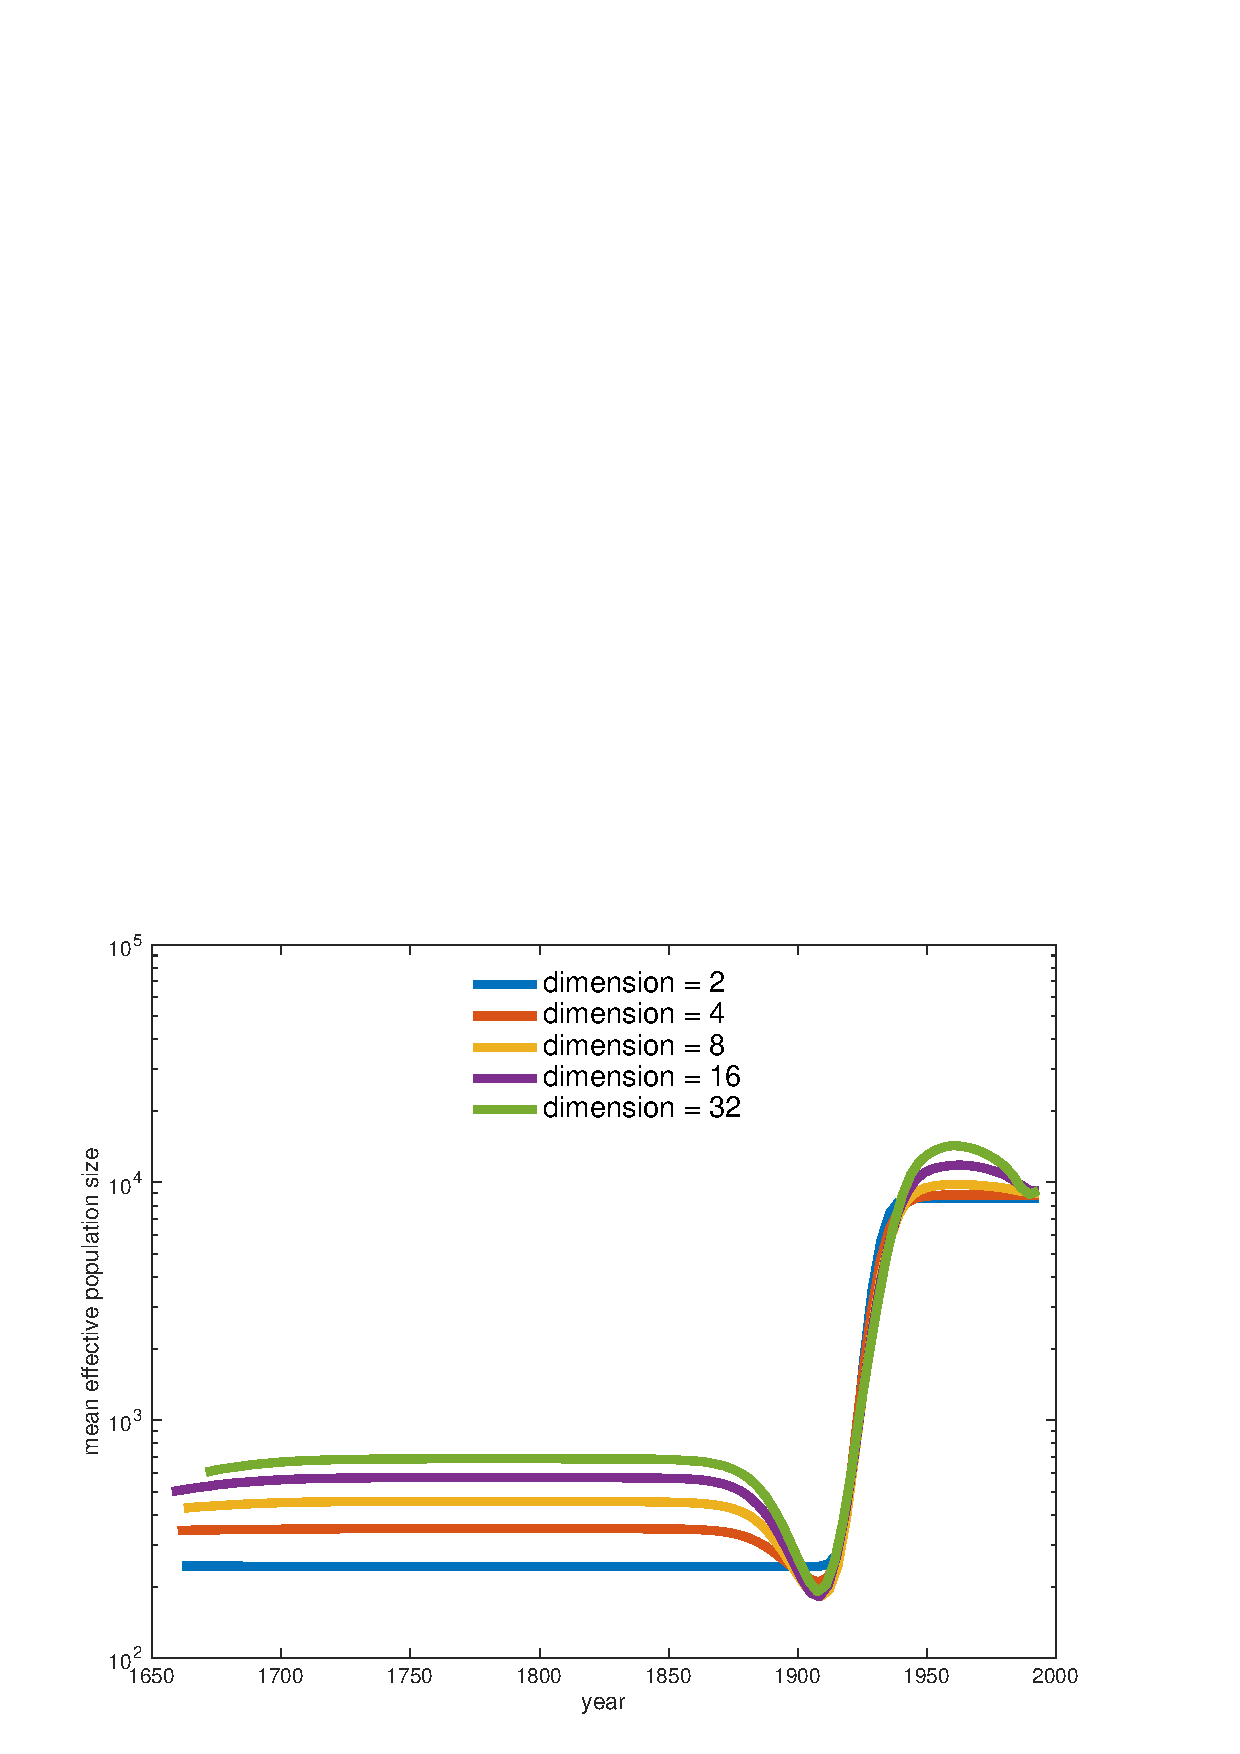
\includegraphics[width=0.500000\textwidth]{figures/comparison_dimension.png}
    \caption{Estimated mean effective population sizes using different dimensions.}
    \label{fig:comparison}
\end{figure}

The choice of the number of dimensions can also have a direct effect on
how fast the MCMC converges (Figure \ref{fig:ess}). The slower
convergence with increasing dimension can be caused by e.g.~less
information in intervals. To some extent it is simply caused by the need
to estimate more parameters though.

\begin{figure}
    \centering
    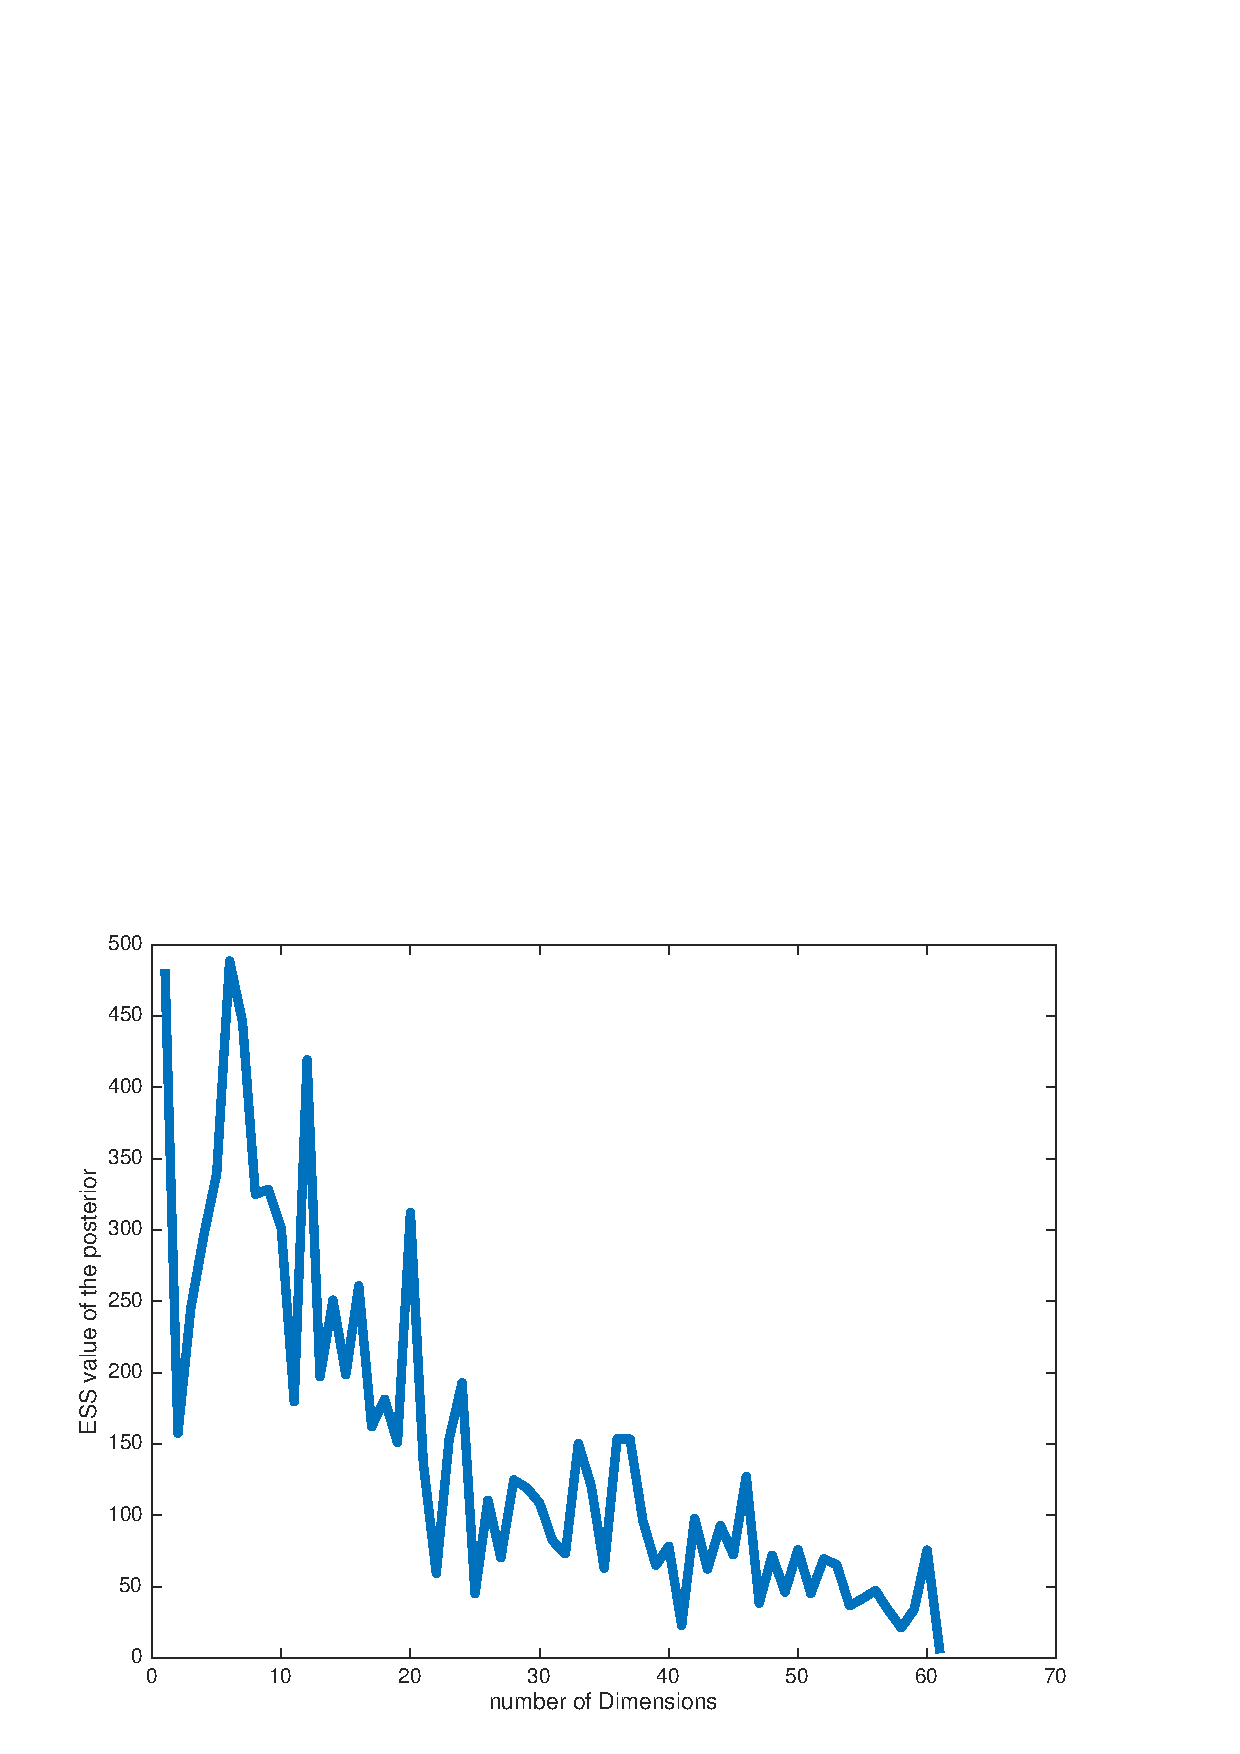
\includegraphics[width=0.500000\textwidth]{figures/ess_vs_dim_coal.png}
    \caption{The ESS value of the posterior after running an MCMC chain with `$ 10^7 $` samples, logged every `$ 10^3 $` steps and a burnin of 10\% for using different dimensions of the Bayesian Coalescent Skyline.}
    \label{fig:ess}
\end{figure}

 \clearpage

\subsubsection{Birth-Death Skyline}\label{birth-death-skyline}

In the first analysis, we used the coalescent approach to estimate
population dynamics, we now want to do the inference using the
birth-death skyline model. We will mostly need the same setups as for
the previous analysis. In case you closed BEAUti, you can reopen the
previously used configuration file in BEAUti (\lstinline!File > Load!
the \lstinline!*.xml!) and modify it to have a birth-death skyline prior
on the tree. We will need to set the prior to
\lstinline!Birth Death Skyline Contemporary!, since the sequences were
all sampled at the same point in time (see Figure \ref{fig:bdsky}). For
samples that were taken through time, we would take
\lstinline!Birth Death Skyline Serial!.

\begin{figure}
    \centering
    \includegraphics[max width=\textwidth, max height=0.9\textheight]{figures/choose_bdsky.png}
    \caption{Setting the prior on the tree to the birth-death skyline.}
    \label{fig:bdsky}
\end{figure}

As in the Bayesian Coalescent Skyline, we need to choose the number of
dimensions. Here we choose the dimensions for the $ R_e $,
the basic reproduction number, which denotes the number of secondary
infections caused by a single infected person in a completely
susceptible population, i.e.~an $ R_e $ of 2 would mean that
every infected person causes two new infections on average. Or in other
words, an $ R_e $ above 1 means that the number of cases are
increasing, therefore the disease will cause an epidemic, and an
$ R_e $ below 1 means that the epidemic will die out. (Note
that since the birth-death skyline infers changes in $ R_e $
over time, it technically infers the effective reproduction number, the
average number of new infections caused by an infected person at a
certain time during the outbreak).

The dimension of the $ R_e $ has to be chosen in the
initialization panel. Choosing this dimension can again be arbitrary and
may require the testing of a few different values. Too few intervals and
not all rate shifts are captured. Too many intervals and the intervals
may not contain enough information to infer parameters.

In this case we will keep the default value of 10 dimensions (Figure
\ref{fig:dimensions_bdsky}).

\begin{figure}
    \centering
    \includegraphics[max width=\textwidth, max height=0.9\textheight]{figures/choose_dimension_bdsky.png}
    \caption{Setting the dimensions for `$ R_e $` estimates.}
    \label{fig:dimensions_bdsky}
\end{figure}

\begin{figure}
    \centering
    \includegraphics[width=0.250000\textwidth]{figures/bdsky_model.png}
    \caption{A schematic of the BDSKY model.}
    \label{fig:bdsky_model}
\end{figure}

BDSKY infers 3 parameters (Figure \ref{fig:bdsky_model}), the
transmission rate $ \lambda $, the becoming noninfectious
rate $ \delta $ and the sampling proportion,
$ \rho $ (when the samples were taken at the same time) or
the sampling proportion, $ p $ (when the samples were taken
through time). The $ R_{0} $ is then a function of those
values (more about that later). The rates we estimate using the
birth-death model are per lineage rates. Some of these rates we know or
we can estimate them from other data. The becoming noninfectious rate
for example, we can get from the average time a patient can transmit a
disease. This prior knowledge we can incorporate in the MCMC. This we
can do in the \lstinline!Priors! panel. We can use prior information
about the $ R_{0} $, the becoming noninfectious rate, the
origin and $ \rho $ (Figures
\protect\hyperlink{fig:r0prior}{14},\protect\hyperlink{fig:bURprior}{15},\protect\hyperlink{fig:oriprior}{16},\protect\hyperlink{fig:rhoprior}{17}).
Note that the origin inferred by the birth-death skyline is not the time
of the most recent common ancestor of the tree (TMRCA), but is earlier
and denotes the start of the outbreak, i.e.~when there was only one
infected person.

We use a lognormal prior for $ R_e $. This is a good prior
distribution to use for rates since it is always positive (a rate cannot
be negative) and has a long tail defined over all positive numbers. The
long tail allows arbitrarily high estimates of $ R_e $, but
does not place much weight on very high rates. This agrees with our
prior knowledge about the $ R_e $ of other diseases (most
diseases have an $ R_e $ between 1.2 and 5. Measles is one
of the most infectious diseases we know about and has an
$ R_e $ of around 18).

If an epidemic is neither growing nor declining, it has an
$ R_e $ of 1, which we will use as a null hypothesis (we
assume that as long as there is no strong signal in an interval for an
epidemic to grow or decline that the $ R_e $ is 1, i.e.~the
epidemic stays constant). Thus, we set the mean of the lognormal
distribution to 0, which results in a median of 1. We set the variance
to 1.25, which places most weight below 7.82 (95\% quantile). (Figure
\ref{fig:r0prior}).

\begin{figure}
    \centering
    \includegraphics[max width=\textwidth, max height=0.9\textheight]{figures/bdsky_prior_r0.png}
    \caption{Setting the `$ R_e $` prior.}
    \label{fig:r0prior}
\end{figure}

For the becoming noninfectious rate we again use a lognormal prior. The
inverse of the becoming noninfectious rate is the average infectious
period. In some patients an HCV infection only lasts a few weeks, while
in others it is a chronic infection lasting for many years. Setting
$ M=0 $ and $ S=1.25 $ results in the same prior
we used for the $ R_e $ (Figure \ref{fig:bURprior}). In
terms of the becoming noninfectious rate, this translates to the 95\%
quantiles for the infectious period falling between 0.128 years (46.67
days) and 11.59 years, with a median of 1 year. We will see later that
there is a strong signal in the data for a longer becoming noninfectious
period.

\begin{figure}
    \centering
    \includegraphics[max width=\textwidth, max height=0.9\textheight]{figures/bdsky_prior_uninf.png}
    \caption{Setting the becoming noninfectious prior.}
    \label{fig:bURprior}
\end{figure}

For the origin of the epidemic we once again use a lognormal prior. Note
that the origin also has to be positive and needs to be bigger than the
MRCA of the tree. We know that HCV has been circulating in Egypt for at
least a hundred years, so we set $ M=5 $ and
$ S=0.5 $ (Figure \ref{fig:oriprior}), resulting in a median
prior estimate for the origin of 148 years.

\begin{figure}
    \centering
    \includegraphics[max width=\textwidth, max height=0.9\textheight]{figures/bdsky_prior_ori.png}
    \caption{Setting the prior on the origin of the epidemic.}
    \label{fig:oriprior}
\end{figure}

Finally, we need a prior for the sampling probability,
$ \rho $, which represents the proportion of HCV cases in
Egypt in 1993, included in the analysis. Egypt had a population of
roughly 60 million in 1993, and with a prevalence of at least 15\% this
translates into millions of cases, whereas we have only 63 sequences.

We use a beta distribution for the prior on $ \rho $. Beta
distributions are a very flexible class of distributions that are only
defined between 0 and 1, making them ideal to use for proportions. We
set Alpha to 1 and Beta to 9999, reflecting our prior knowledge that we
have only a minuscule fraction of all cases in our dataset (Figure
\ref{fig:rhoprior}).

\begin{figure}
    \centering
    \includegraphics[max width=\textwidth, max height=0.9\textheight]{figures/bdsky_prior_rho.png}
    \caption{Setting the prior on `$ \rho $`.}
    \label{fig:rhoprior}
\end{figure}

We can leave the rest of the priors as they are. First, we should
increase the chain length (at least double it). To not get too large log
files, we can increase the \lstinline!sampling every! to 2000 (reducing
the sampling frequency). Now we can change the names of the output
files. If we want to run the analysis in the same directory as the
coalescent analyses, the output files and the \lstinline!*.xml! name
need to be different.

\subsubsection{The parameterization of the Birth-Death
Model}\label{the-parameterization-of-the-birth-death-model}

The Birth-Death model is parameterized very differently from the
coalescent model. While the coalescent uses the effective population
size, which as the name already tells us is defined on a population
level, the birth-death model uses per lineage rates. The transmission
rate $ \lambda $ tells us at which rate infected individuals
infect susceptibles. This rate is also referred to as the birth rate.
The sampling rate $ \psi $ and the sampling probability
$ \rho $ describe how likely it is for an infected
individual to be sampled and therefore how likely they are to appear in
the tree as tips. The becoming noninfectious rate $ \delta $
is the sum of the death rate $ \mu $ and the sampling rate
$ \psi $.

\begin{equation}
    \delta = \psi + \mu
\end{equation}

The death rate $ \mu $ is the rate at which lineages
disappear (go extinct) from a population without being sampled. You can
also see from the above equation that we assume that a sampled lineage
cannot transmit anymore. The consequence for the phylogeny is that a
sampled lineage cannot be an ancestor of any lineage. This assumption
can be relaxed, but we will not do so during this tutorial.

The $ R_e $ we estimate is then defined as follows:

\begin{equation}
    R_{0} = \frac{\lambda}{\psi + \mu} = \frac{\lambda}{\delta}
\end{equation}

\begin{longtable}[]{@{}rl@{}}

if $ \lambda > \delta $ then $ R_e > 1 $ &
epidemic grows\tabularnewline
if $ \lambda = \delta $ then $ R_e = 1 $ &
epidemic stays constant\tabularnewline
if $ \lambda < \delta $ then $ R_e < 1 $ &
epidemic declines\tabularnewline

\end{longtable}

The birth-death skyline allows these rates to change over time. This is
done by dividing the time from the origin (of the epidemic, which is not
necessarily the same as the root of the tree) to the most recent sample
into dimension $ d $ equally spaced intervals (see Figure
\ref{fig:bdsky_principle}). The rates are then allowed to change between
two intervals. Within an interval rates are constant. In principle, all
rates in all intervals could be different. Since the transmission rate
and the becoming noninfectious rate are highly correlated, this is not
always practical. Often we assume the becoming noninfectious rate to be
the same in all intervals while changing the transmission rate
$ \lambda $.

\begin{figure}
    \centering
    \includegraphics[width=0.500000\textwidth]{figures/bdsky_intervals5.png}
    \caption{Example tree where the red dotted lines are an example of where rates could be allowed to change on the tree. The branch at the root (compare Figure 6) is indicating the origin of the epidemic, which is also estimated in the BDSKY.}
    \label{fig:bdsky_principle}
\end{figure}

There are some clear differences between the birth-death and the
coalescent skyline. First, the way intervals are defined. In the
coalescent skyline, intervals are always between coalescent events,
while this restriction does not exist for the birth-death skyline.
Second, the birth-death skyline does not infer changes in population
sizes.

The coalescent on the other hand does infer the effective population
size, which is a parameter proportional to absolute sizes. The third
difference is the inference of the origin of an epidemic by the birth
death model, which is not done by the coalescent.

\subsubsection{Visualizing the Birth-Death Skyline
Output}\label{visualizing-the-birth-death-skyline-output}

There is no equivalent visualization of the \lstinline!*.log! file of a
BDSKY analysis in tracer as there is for the Bayesian Coalescent
Skyline. But because BDSKY separates the full tree into equally spaced
intervals, we can already get an idea of the inference just by looking
at the inferred $ R_e $ values (see Figure
\ref{fig:bdsky_dynamics}). This gives us a good idea of the trend, but
it is not completely accurate. Since every posterior sample has a
different origin, the time spanned by each interval is slightly
different in each posterior sample. Thus, the different intervals
overlap slightly. The advantage to this is that we get a smooth estimate
through time. The disadvantage is that we need to do some extra
post-processing to plot the skyline.

\begin{figure}
    \centering
    \includegraphics[max width=\textwidth, max height=0.9\textheight]{figures/bdsky_tracer.png}
    \caption{Estimated population dynamics by BDSKY in Tracer.}
    \label{fig:bdsky_dynamics}
\end{figure}

We will instead use the R package \lstinline!bdskytools! to plot the
output of the bdsky. The package is still in development and currently
not available over CRAN. Thus, we have to install the package directly
over GitHub (note that you only have to install the package once):

\begin{lstlisting}
install.packages("devtools")
library(devtools)

devtools::install_github("laduplessis/bdskytools")
\end{lstlisting}

Once the package is installed we have to load the package into our R
workspace before we can use the functions in the package. To plot the
results, we need to tell R where to find the \lstinline!*.log! file of
our run and load it into R (discarding 10\% of samples as burn-in):

\begin{lstlisting}
library(bdskytools)

fname <- "Replace this string with the path to your log file"
lf    <- readLogfile(fname, burnin=0.1)
\end{lstlisting}

Next, we can extract the HPDs of $ R_e $ and the becoming
noninfectious rate:

\begin{lstlisting}
Re_sky    <- getSkylineSubset(lf, "reproductiveNumber")
Re_hpd    <- getMatrixHPD(Re_sky)
delta_hpd <- getHPD(lf$becomeUninfectiousRate)
\end{lstlisting}

Next we plot the raw HPD intervals of $ R_e $. This is
equivalent to the output in tracer.

\begin{lstlisting}[language=R]
plotSkyline(1:10, Re_hpd, type='step', ylab="R")
\end{lstlisting}

\begin{figure}
    \centering
    \includegraphics[width=0.800000\textwidth]{figures/bdsky_hpds.png}
    \caption{The HPDs of `$ R_e $` (equivalent to the previous figure).}
    \label{fig:bdsky_hpds}
\end{figure}

In order to plot the smooth skyline we have to calculate the HPD on a
finer timegrid. To do this we first calculate the marginal posterior at
every time of interest using the function \lstinline!gridSkyline! and
then calculate the HPD for each of the finer time intervals. The times
to grid the skyline on (\lstinline!timegrid!), refers to years in the
past.

\begin{lstlisting}[language=R]
timegrid <- seq(1,400,length.out=100)
Re_gridded     <- gridSkyline(Re_sky, lf$origin, timegrid)
Re_gridded_hpd <- getMatrixHPD(Re_gridded)
\end{lstlisting}

Now we are ready to plot the smooth skyline (remember that the sequences
were sampled in 1993):

\begin{lstlisting}[language=R]
times     <- 1993-timegrid
plotSkyline(times, Re_gridded_hpd, type='smooth', xlab="Time", ylab="R")
\end{lstlisting}

\begin{figure}
    \centering
    \includegraphics[width=0.800000\textwidth]{figures/bdsky_smooth.png}
    \caption{The smooth `$ R_e $` skyline.}
    \label{fig:bdsky_smooth}
\end{figure}

We can plot the gridded skyline (not its HPDs) for a few of the samples
to see what it really looks like. Note that the intervals overlap
between different posterior samples. This is because the origin is
different in each sample. As we add more samples to the plot we start to
see the smooth skyline appear.

\begin{lstlisting}[language=R]
plotSkyline(times, Re_gridded, type='steplines', traces=10, col=pal.dark(cblue,0.5),ylims=c(0,5), xlab="Time", ylab="R")
plotSkyline(times, Re_gridded, type='steplines', traces=100, col=pal.dark(cblue,0.5),ylims=c(0,5), xlab="Time", ylab="R")
plotSkyline(times, Re_gridded, type='steplines', traces=1000, col=pal.dark(cblue,0.1),ylims=c(0,5), xlab="Time", ylab="R")
\end{lstlisting}

\begin{figure}
    \centering
    \includegraphics[width=0.800000\textwidth]{figures/bdsky_traces.png}
    \caption{Increasing the number of traces plotted from 10 to 100, to 1000.}
    \label{fig:bdsky_traces}
\end{figure}

Finally, we can plot both the $ R_e $ and the becoming
noninfectious rate on a single set of axes. Since we left the dimension
of the becoming noninfectious rate at 1, it is constant through time.
(Normally we would not plot constant parameters over a time period). The
output should be similar to Figure \ref{fig:bdsky_out}.

\begin{lstlisting}[language=R]
par(mar=c(5,4,4,4)+0.1)

plotSkylinePretty(range(times), as.matrix(delta_hpd), type='step', axispadding=0.0, col=pal.dark(cblue), fill=pal.dark(cblue, 0.5), col.axis=pal.dark(cblue),
ylab=expression(delta), side=4, yline=2, ylims=c(0,1), xaxis=FALSE)

plotSkylinePretty(times, Re_gridded_hpd, type='smooth', axispadding=0.0, col=pal.dark(corange), fill=pal.dark(corange, 0.5), col.axis=pal.dark(corange),
xlab="Time", ylab=expression("R"[e]), side=2, yline=2.5, xline=2, xgrid=TRUE, ygrid=TRUE, gridcol=pal.dark(cgray), ylims=c(0,3), new=TRUE, add=TRUE)
\end{lstlisting}

\begin{figure}
    \centering
    \includegraphics[width=0.800000\textwidth]{figures/bdsky_output.png}
    \caption{Estimates of the inferred `$ R_e $` (orange) over time and the estimate of the becoming un-infectious rate (blue), for which we only used one value.}
    \label{fig:bdsky_out}
\end{figure}

An R script with the above commands (and a few extras) is in the
\lstinline!scripts/! directory (\lstinline!Skyline_Example.R!). If the
bdskytools package cannot be installed from GitHub the relevant scripts
are also provided in the \lstinline!scripts/! directory.

\clearpage

\subsection{Some considerations for using skyline
plots}\label{some-considerations-for-using-skyline-plots}

Both the coalescent and the birth-death skylines assume that the
population is well-mixed. That is, they assume that there is no
significant population structure and that the sequences are a random
sample from the population. However, if there is population structure,
for instance sequences were sampled from two different villages and
there is much more contact within than between villages, then the
results will be biased \citep{Heller2013}. Instead a structured model
should be used to account for these biases.

\clearpage

\section{Useful Links}\label{useful-links}

\begin{itemize}

\item
  \href{http://www.beast2.org/book.html}{Bayesian Evolutionary Analysis
  with BEAST 2} \citep{BEAST2book2014}
\item
  BEAST 2 website and documentation: \url{http://www.beast2.org/}
\item
  BEAST 1 website and documentation: \url{http://beast.bio.ed.ac.uk}
\item
  Join the BEAST user discussion:
  \url{http://groups.google.com/group/beast-users} \clearpage
\end{itemize}



%%%%%%%%%%%%%%%%%%%%%%%
% Tutorial disclaimer %
%%%%%%%%%%%%%%%%%%%%%%%
% Please do not change the license
% Add the author names and relevant links
% Add any other aknowledgments here
\href{http://creativecommons.org/licenses/by/4.0/}{\includegraphics[scale=0.8]{figures/ccby.pdf}} This tutorial was written by Nicola F. Müller and Louis du Plessis for \href{https://taming-the-beast.github.io}{Taming the BEAST} and is licensed under a \href{http://creativecommons.org/licenses/by/4.0/}{Creative Commons Attribution 4.0 International License}. 


%%%%%%%%%%%%%%%%%%%%
% Do NOT edit this %
%%%%%%%%%%%%%%%%%%%%
Version dated: \today



\newpage

%%%%%%%%%%%%%%%%
%  REFERENCES  %
%%%%%%%%%%%%%%%%

\printbibliography[heading=relevref]


\end{document}